\chapter{Solutions for Linear Systems}
\label{chap:SolLinSys}

The last chapter introduced the necessary machinery for solving linear systems of equations, and now we are going to see how to apply those methods (Gaussian Elimination and Inverse) under suitable circumstances. We will first study how to solve linear systems mathematically, and then move to the application parts at the end. Remember, in the first chapter, we formulated some problems about linear systems of equations appearing in Earth Science, such as seismic tomography and radiative transfer in the atmosphere, and they will be addressed accordingly.

\section{Number of Solutions for Linear Systems}
\label{section:NoSolLinSys}

Before tackling any linear system, we may like to know how many solutions there are. In fact, there are only three possibilities.
\begin{thm}[Number of Solutions for a Linear System]
For a system of linear equations $A\vec{x} = \smash{\vec{h}}$ (recall Definition \ref{defn:linsys} and Properties \ref{proper:linsysmat}), it has either:
\begin{enumerate}
\item No solution,
\item A unique solution, or
\item Infinitely many solutions.
\end{enumerate}
for the unknowns $\vec{x}$.
\end{thm}
This can be illustrated by considering a linear system with two equations and two unknowns, with each equation representing a line. There are three types of scenarios, shown in Figure \ref{fig:2dlinsysdemo} below.
\begin{align}
\label{eqn:2dlinsysdemo}
\left\{\begin{alignedat}{1}
a_1x + b_1y &= h_1 \\
a_2x + b_2y &= h_2
\end{alignedat}\right.
\end{align}
It goes similarly for any linear system of three unknowns in which equations represent planes instead, and the intersection of two non-parallel planes will be a line. We show three possible scenarios in Figure \ref{fig:3dlinsysdemo} (notice the central panel represents a non-square $2 \times 3$ system). The readers can try to imagine and draw out other possibilities.
\begin{figure}[hb!]
\centering
\begin{subfigure}{0.7\textwidth}
\centering
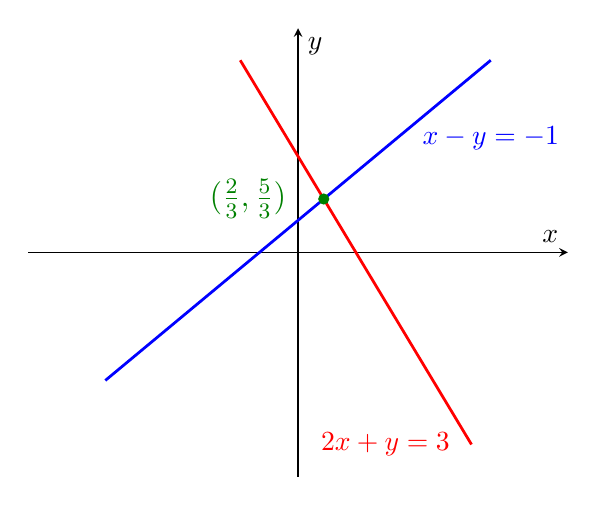
\begin{tikzpicture}
\begin{axis}
[axis y line=middle,
axis x line=middle,
xlabel=$x$,ylabel=$y$,
enlargelimits=0.2,
xmin=-5,xmax=5,
ymin=-5,ymax=5,ticks=none]
\addplot[mark=none, color=blue, line width=1] {x+1} node[below, yshift=-20]{$x-y=-1$};
\addplot[mark=none, color=red, line width=1, domain=-1.5:4.5] {-2*x+3} node[left, xshift=-4]{$2x+y=3$};
\addplot[mark=*, color=Green, mark size=1.8pt] coordinates {(2/3, 5/3)} node[left, xshift=-10]{\large$(\frac{2}{3}, \frac{5}{3})$};
\end{axis}
\end{tikzpicture} 
\caption{\textit{One solution: Two non-parallel lines (red/blue) intersecting at one point (green).}}
\end{subfigure}
\end{figure}
\begin{figure}[ht!]
\ContinuedFloat
\centering
\begin{subfigure}{0.7\textwidth}
\centering
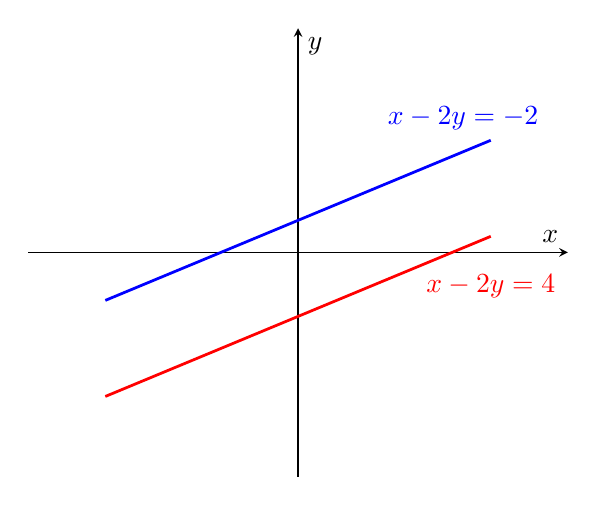
\begin{tikzpicture}
\begin{axis}
[axis y line=middle,
axis x line=middle,
xlabel=$x$,ylabel=$y$,
enlargelimits=0.2,
xmin=-5,xmax=5,
ymin=-5,ymax=5,ticks=none]
\addplot[mark=none, color=blue, line width=1] {1/2*x+1} node[above, xshift=-10]{$x - 2y = -2$};
\addplot[mark=none, color=red, line width=1] {1/2*x-2} node[below, yshift=-10]{$x - 2y = 4$};
\end{axis}
\end{tikzpicture}
\caption{\textit{No solution: Two parallel lines never touch each other.}}
\end{subfigure}
\begin{subfigure}{0.7\textwidth}
\centering
\begin{tikzpicture}
\begin{axis}
[axis y line=middle,
axis x line=middle,
xlabel=$x$,ylabel=$y$,
enlargelimits=0.2,
xmin=-5,xmax=5,
ymin=-5,ymax=5,ticks=none]
\addplot[mark=none, color=Green, line width=1, domain=-2.25:0.875] {-4*x-3};
\node[blue] at (-4,2) {$4x+y=-3$};
\node[red] at (3,-3) {$8x+2y=-6$};
\end{axis}
\end{tikzpicture}
\caption{Infinitely many solutions: Two parallel lines overlap each other.}
\end{subfigure}
\caption{\textit{Three possible situations for (\ref{eqn:2dlinsysdemo}).}}
\label{fig:2dlinsysdemo}
\end{figure}
\begin{figure}[ht!]
    \centering
    \begin{minipage}{0.32\textwidth}
    \centering
    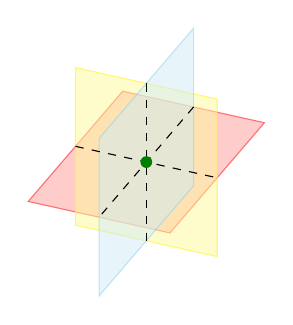
\begin{tikzpicture}[x={(-0.9cm, 0.2cm)}, y={(0.6cm, 0.7cm)}, z={(0cm, 1cm)}]
    \filldraw[draw=Red, fill=Red!40, opacity=0.5]
    (-1,-1,0) -- (-1,1,0) -- (1,1,0) -- (1,-1,0) -- cycle;
    \filldraw[draw=yellow, fill=yellow!40, opacity=0.5]
    (-1,0,-1) -- (-1,0,1) -- (1,0,1) -- (1,0,-1) -- cycle;
    \filldraw[draw=SkyBlue, fill=SkyBlue!40, opacity=0.5]
    (0,-1,-1) -- (0,-1,1) -- (0,1,1) -- (0,1,-1) -- cycle;
    \draw[dashed] (1,0,0) -- (-1,0,0);
    \draw[dashed] (0,1,0) -- (0,-1,0);
    \draw[dashed] (0,0,1) -- (0,0,-1);
    \node at (0,0,0) [circle,fill,inner sep=1.5pt,Green]{};
    \end{tikzpicture} \\
    \end{minipage}
    \begin{minipage}{0.32\textwidth}
    \centering
    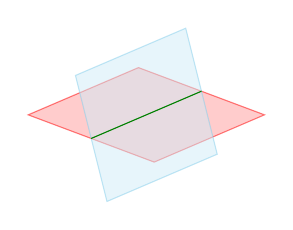
\begin{tikzpicture}[x={(-0.8cm, 0.3cm)}, y={(0.7cm, 0.3cm)}, z={(-0.2cm, 0.8cm)}]
    \filldraw[draw=Red, fill=Red!40, opacity=0.5]
    (-1,-1,0) -- (-1,1,0) -- (1,1,0) -- (1,-1,0) -- cycle;
    \filldraw[draw=SkyBlue, fill=SkyBlue!40, opacity=0.5]
    (0,-1,-1) -- (0,-1,1) -- (0,1,1) -- (0,1,-1) -- cycle;
    \draw[Green] (0,1,0) -- (0,-1,0);
    \end{tikzpicture} \\
    \end{minipage}
    \begin{minipage}{0.32\textwidth}
    \centering
    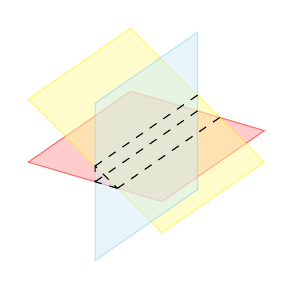
\begin{tikzpicture}[x={(-0.85cm, 0.25cm)}, y={(0.65cm, 0.45cm)}, z={(0cm, 1cm)}]
    \filldraw[draw=Red, fill=Red!40, opacity=0.5]
    (-1,-1,0) -- (-1,1,0) -- (1,1,0) -- (1,-1,0) -- cycle;
    \filldraw[draw=yellow, fill=yellow!40, opacity=0.5]
    (-1,-1,-0.4) -- (-1,1,-0.4) -- (1,1,0.8) -- (1,-1,0.8) -- cycle;
    \filldraw[draw=SkyBlue, fill=SkyBlue!40, opacity=0.5]
    (0,-1,-1) -- (0,-1,1) -- (0,1,1) -- (0,1,-1) -- cycle;
    \draw[dashed] (0,1,0.2) -- (0,-1,0.2);
    \draw[dashed] (0,1,0) -- (0,-1,0);
    \draw[dashed] (-0.333,1,0) -- (-0.333,-1,0);
    \draw[dashed] (-0.333,-1,0) -- (0,-1,0) -- (0,-1,0.2) -- cycle;
    \end{tikzpicture}
    \end{minipage}
    \caption{\textit{One solution (left): Three planes (red/yellow/blue) intersecting at one point (green). Infinitely many solutions (middle): Two planes intersecting along a straight line. No solution (right): Three planes intersecting pairwise along three parallel lines that do not intersect.}}
    \label{fig:3dlinsysdemo}
\end{figure}

In fact, this theorem about the existence of solutions is true for any number of variables and equations.\footnotemark{} If there is any solution, then the system is called \index{Consistent}\keywordhl{consistent}. Otherwise, if no solution exists, then it is known as \index{Inconsistent}\keywordhl{inconsistent}.\par

Clearly, the next task is to find out which case the linear system belongs to. The following theorem reveals the relationship between the number of solutions for a \textit{square} linear system and the determinant of its coefficient matrix.
\begin{thm}
\label{thm:sqlinsysunique}
For a square linear system $A\vec{x} = \vec{h}$, if the coefficient matrix $A$ is invertible, i.e.\ $\det(A) \neq 0$, then there is always only one unique solution. However, if $A$ is singular, $\det(A) = 0$, then it has either no solution, or infinitely many solutions.
\end{thm}
\footnotetext{Some readers may think if there can be finitely many solutions only. Unfortunately, it is impossible. Assume there are two distinct solutions $\vec{x}^{(1)}$, $\vec{x}^{(2)}$ to the system $A\vec{x} = \smash{\vec{h}}$, then it is easy to show by construction all $\vec{x}_t = t\vec{x}^{(1)} + (1-t)\vec{x}^{(2)}$ for any $t$ will be valid solutions which are infinitely many.}As a consequence, if the homogeneous linear system $A\vec{x} = \textbf{0}$ has a singular coefficient matrix with $\det(A) = 0$, since it always has a trivial solution of $\vec{x} = \textbf{0}$, the above theorem implies that the homogeneous system must have infinitely many solutions (because it cannot have no solution). We defer the arguments for showing Theorem \ref{thm:sqlinsysunique}, as well as the discussion about non-square systems, until we actually start solving linear systems in the next subsection. \par
$\blacktriangleright$ Short Exercise: By inspection, determine the number of solutions for the following linear systems.\footnotemark
\begin{align*}
&
\begin{bmatrix}
2 & 1 & 6 \\
3 & 0 & 4 \\
1 & 1 & 5 
\end{bmatrix}
\begin{bmatrix}
x \\
y \\
z
\end{bmatrix}
=
\begin{bmatrix}
0 \\
0 \\
0
\end{bmatrix}
&
\begin{bmatrix}
1 & 4 & 3 \\
1 & 5 & 2 \\
1 & 3 & 4 
\end{bmatrix}
\begin{bmatrix}
x \\
y \\
z
\end{bmatrix}
=
\begin{bmatrix}
0 \\
0 \\
0
\end{bmatrix}
\end{align*}

\section{Solving Linear Systems}
\label{section:SolveLinSys}
Now it is time to get down to solving linear systems (preferably written in matrix form), and we have two methods to choose from:
\begin{enumerate}
\item By Gaussian Elimination, for linear systems in any shape, or
\item By Inverse, which is apparently only applicable for square, invertible coefficient matrices.
\end{enumerate}

\subsection{Solving Linear Systems by Gaussian Elimination}
\label{subsection:SolLinSysGauss}

Like in Section \ref{subsection:invGauss}, applying Gaussian Elimination on the augmented matrix (introduced at the end of Section \ref{section:deflinsys}) of a linear system can yield the solution to the right. The principle involving elementary row operations is the same as that in Definition \ref{defn:elementarymat} and Theorem \ref{thm:Gausselimprincip}, but with $A\vec{x} = \smash{\vec{h}}$ instead of $AA^{-1} = I$. Let $A_{\text{rref}}$ be the reduced row echelon form of $A$, and $E_1, E_2, \ldots, E_n$ be the elementary matrices used in the Gaussian Elimination process to arrive at the RREF. For any solution $\vec{x}$ to the system $A\vec{x} = \smash{\vec{h}}$, we multiply the elementary matrices one by one to the left on both sides of the equation, leading to
\begin{align}
(E_n\cdots E_2E_1)A\vec{x} &= (E_n\cdots E_2E_1)\vec{h} \nonumber \\
(E_n\cdots E_2E_1A)\vec{x} = A_{\text{rref}}\vec{x} &= (E_n\cdots E_2E_1)\vec{h} 
\end{align}
hence $\vec{x}$ will be the solution to $A_{\text{rref}}\vec{x} = \tilde{h}$ too at the same time, where $\smash{\tilde{h}} = E_n\cdots E_2E_1\smash{\vec{h}}$. Therefore, the solutions of $A\vec{x} = \smash{\vec{h}}$ and $A_{\text{rref}}\vec{x} = \smash{\tilde{h}}$ coincide, which can be inferred more directly from the latter reduced system. In addition, the coefficient matrix $A$ can be non-square, but we will look at the easier case of a square coefficient matrix first.\footnotetext{The coefficient matrices of these two homogeneous linear systems have determinants of $-1$ and $0$ respectively, and hence by Theorem \ref{thm:sqlinsysunique}, the first system has a unique solution and the second one has infinitely many solutions.}

\subsubsection{Square Systems}
\begin{exmp}
Solve the following linear system using Gaussian Elimination.
\begin{align*}
\begin{bmatrix}
1 & 0 & 1 \\
1 & 1 & 4 \\
2 & 0 & 3
\end{bmatrix}
\begin{bmatrix}
x \\
y \\
z
\end{bmatrix}
=
\begin{bmatrix}
3 \\
10 \\
8
\end{bmatrix}
\end{align*}
\end{exmp}
\begin{solution}
We rewrite the system in augmented form and then apply Gaussian Elimination, with the aim of reducing the coefficient matrix on the left to the identity matrix.
\begin{align*}
\left[\begin{array}{@{\,}wc{10pt}wc{10pt}wc{10pt}|wc{10pt}@{\,}}
1 & 0 & 1 & 3 \\
1 & 1 & 4 & 10 \\
2 & 0 & 3 & 8
\end{array}\right] 
& \to 
\left[\begin{array}{@{\,}wc{10pt}wc{10pt}wc{10pt}|wc{10pt}@{\,}}
1 & 0 & 1 & 3 \\
0 & 1 & 3 & 7 \\
0 & 0 & 1 & 2
\end{array}\right] 
& \begin{aligned}
R_2-R_1 &\to R_2 \\
R_3-2R_1 &\to R_3 
\end{aligned} \\
& \to 
\left[\begin{array}{@{\,}wc{10pt}wc{10pt}wc{10pt}|wc{10pt}@{\,}}
1 & 0 & 0 & 1 \\
0 & 1 & 0 & 1 \\
0 & 0 & 1 & 2
\end{array}\right] 
& 
\begin{aligned}
R_2-2R_3 &\to R_2 \\
R_1-R_3 &\to R_1    
\end{aligned}
\end{align*}
which translates to
\begin{align*}
&
\begin{cases}
x = 1 \\
y = 1 \\
z = 2
\end{cases}
& \text{or} &
& \vec{x} = 
\begin{bmatrix}
x \\
y \\
z
\end{bmatrix}
=
\begin{bmatrix}
1 \\
1 \\
2
\end{bmatrix}
\end{align*}
Note that we have successfully converted the coefficient matrix to the identity along the way, which by (c) to (a) in Theorem \ref{thm:equiv1}, implies that the coefficient matrix is invertible. This explains the first part of Theorem \ref{thm:sqlinsysunique}, as every unknown is now associated with a single leading $1$ in the corresponding column of the identity matrix acquired from the Gaussian reduction process, and a unique solution can be derived.
\end{solution}

\begin{exmp}
\label{exmp:nosol}
Solve the linear system
\begin{align*}
\begin{bmatrix}
3 & 7 & 2 \\
1 & 1 & 0 \\
0 & 2 & 1 
\end{bmatrix}
\begin{bmatrix}
x \\
y \\
z
\end{bmatrix}
=
\begin{bmatrix}
8 \\
2 \\
2
\end{bmatrix}   
\end{align*}
if possible.
\end{exmp}
\begin{solution} Again, we apply Gaussian Elimination on the augmented matrix to obtain
\begin{align*}
\left[\begin{array}{@{\,}wc{10pt}wc{10pt}wc{10pt}|wc{10pt}@{\,}}
3 & 7 & 2 & 8 \\
1 & 1 & 0 & 2 \\
0 & 2 & 1 & 2
\end{array}\right] 
& \to 
\left[\begin{array}{@{\,}wc{10pt}wc{10pt}wc{10pt}|wc{10pt}@{\,}}
1 & 1 & 0 & 2 \\
3 & 7 & 2 & 8 \\
0 & 2 & 1 & 2
\end{array}\right] 
& R_1 \leftrightarrow R_2 \\
& \to 
\left[\begin{array}{@{\,}wc{10pt}wc{10pt}wc{10pt}|wc{10pt}@{\,}}
1 & 1 & 0 & 2 \\
0 & 4 & 2 & 2 \\
0 & 2 & 1 & 2
\end{array}\right] 
& R_2-3R_1 \to R_2 \\
& \to 
\left[\begin{array}{@{\,}wc{10pt}wc{10pt}wc{10pt}|wc{10pt}@{\,}}
1 & 1 & 0 & 2 \\
0 & 1 & \frac{1}{2} & \frac{1}{2} \\
0 & 2 & 1 & 2
\end{array}\right] 
& \frac{1}{4}R_2 \to R_2 \\
& \to 
\left[\begin{array}{@{\,}wc{10pt}wc{10pt}wc{10pt}|wc{10pt}@{\,}}
1 & 1 & 0 & 2 \\
0 & 1 & \frac{1}{2} & \frac{1}{2} \\
0 & 0 & 0 & 1
\end{array}\right] 
& R_3 - 2R_2 \to R_3
\end{align*}
The last row corresponds to $0 = 1$ which is contradictory. As a consequence, the system is inconsistent, i.e.\ no solution exists.
\end{solution}

\begin{exmp}
\label{exmp:mulsol}
Find all solutions for the following linear system.
\begin{align*}
\begin{bmatrix}
1 & 2 & 1 \\
2 & 5 & 3 \\
0 & 1 & 1 
\end{bmatrix}
\begin{bmatrix}
x \\
y \\
z
\end{bmatrix}
=
\begin{bmatrix}
1 \\
2 \\
0
\end{bmatrix}   
\end{align*}
\end{exmp}
\begin{solution} 
Gaussian Elimination leads to
\begin{align*}
\left[\begin{array}{@{\,}wc{10pt}wc{10pt}wc{10pt}|wc{10pt}@{\,}}
1 & 2 & 1 & 1 \\
2 & 5 & 3 & 2 \\
0 & 1 & 1 & 0
\end{array}\right] 
& \to 
\left[\begin{array}{@{\,}wc{10pt}wc{10pt}wc{10pt}|wc{10pt}@{\,}}
1 & 2 & 1 & 1 \\
0 & 1 & 1 & 0 \\
0 & 1 & 1 & 0
\end{array}\right] 
& R_2 - 2R_1 \to R_2 \\
& \to 
\left[\begin{array}{@{\,}wc{10pt}wc{10pt}wc{10pt}|wc{10pt}@{\,}}
1 & 0 & -1 & 1 \\
0 & 1 & 1 & 0 \\
0 & 0 & 0 & 0
\end{array}\right] 
& \begin{aligned}
R_3-R_2 &\to R_3 \\
R_1-2R_2 &\to R_1    
\end{aligned}
\end{align*}
Now, the last row corresponds to $0 = 0$, which is vacuous and implies that one equation is spurious. This also means that we can assign an unknown as a \index{Free Variable/Parameter}\keywordhl{free variable (parameter)} for expressing other variables. We will choose unknown(s) that is/are not linked to any pivot in the reduced coefficient matrix. As the variables $x$ and $y$ already correspond to the two pivots in the first/second column, we can let $z = t$ where $t$ represents the free parameter. Then the first/second row gives $x = 1+t$, $y = -t$ respectively, and
\begin{align*}
\vec{x} = 
\begin{bmatrix}
x \\
y \\
z
\end{bmatrix}
=
\begin{bmatrix}
1+t \\
-t \\
t
\end{bmatrix}
=
\begin{bmatrix}
1 \\
0 \\
0
\end{bmatrix}
+ t
\begin{bmatrix}
1 \\
-1 \\
1
\end{bmatrix}
\end{align*}
with $-\infty < t < \infty$. The first column vector that appears alone
\begin{align*}
\begin{bmatrix}
1 \\
0 \\
0
\end{bmatrix}    
\end{align*}
is the so-called \index{Particular Solution}\keywordhl{particular solution}, which can be any vector $\vec{x} = \vec{x}_p$ that satisfies the inhomogeneous part of the system $A\vec{x} = \smash{\vec{h}}$. Meanwhile, the second column vector, multiplied by the free parameter $t$
\begin{align*}
t
\begin{bmatrix}
1 \\
-1 \\
1
\end{bmatrix}    
\end{align*}
is known as the \index{Complementary Solution}\keywordhl{complementary solution}, the family of all vectors $\vec{x} = \vec{x}_c$ that satisfy the homogeneous part $A\vec{x} = \textbf{0}$. Combined, they form the \index{General Solution}\keywordhl{general solution} $\vec{x}_g = \vec{x}_p + \vec{x}_c$ as the complete set of solutions to the linear system. 
\end{solution}
$\blacktriangleright$ Short Exercise: Try plugging in any number $t$ to the general solution and verify the consistency.\footnotemark\par
The complementary solution encompasses all possible solutions to the homogeneous part $A\vec{x} = \textbf{0}$ of the linear system $A\vec{x} = \smash{\vec{h}}$. For broader situations, it can contain more than one pair of free parameters and column vectors (or none, if the homogeneous part only permits the trivial solution of all zeros), and the complementary solution becomes a \textit{linear combination} of multiple \textit{linearly independent} column vectors which satisfy $A\vec{x} = \textbf{0}$ on their own. (We will clarify these concepts in Chapter \ref{chap:vec_space}.)\par
The amount of free variables is decided by the number of columns in the coefficient matrix (unknowns), minus the number of pivots (constraints) in its reduced row echelon form. This quantity is called \textit{nullity} and in the last example, it equals $1$. In the case of multiple free variables, we assign the corresponding number of free parameters to non-pivotal unknowns and apply the same procedure as in the example above to acquire the full complementary solution. Any column vector that constitutes the complementary solution (followed by a free parameter) can be scaled by any non-zero factor as we desire.\footnotetext{\label{footnote:3.3}Let's say $t=1$ and $\tilde{x} = 
\begin{bmatrix}
1 \\
0 \\
0
\end{bmatrix}
+ (1)
\begin{bmatrix}
1 \\
-1 \\
1
\end{bmatrix}
=
\begin{bmatrix}
2 \\
-1 \\
1
\end{bmatrix}$, then clearly $A\tilde{x} = 
\begin{bmatrix}
1 & 2 & 1 \\
2 & 5 & 3 \\
0 & 1 & 1 
\end{bmatrix}
\begin{bmatrix}
2 \\
-1 \\
1
\end{bmatrix}
= 
\begin{bmatrix}
1 \\
2 \\
0
\end{bmatrix}$. $\tilde{x}$ can become a new particular solution by noting that the original solution form can be rewritten as
\begin{align*}
\vec{x} =
\begin{bmatrix}
1 \\
0 \\
0
\end{bmatrix}
+ t
\begin{bmatrix}
1 \\
-1 \\
1
\end{bmatrix}
= 
\begin{bmatrix}
1 \\
0 \\
0
\end{bmatrix}
+ (1)
\begin{bmatrix}
1 \\
-1 \\
1
\end{bmatrix}
+
(t-1)
\begin{bmatrix}
1 \\
-1 \\
1
\end{bmatrix}
=
\begin{bmatrix}
2 \\
-1 \\
1
\end{bmatrix}
+
t'
\begin{bmatrix}
1 \\
-1 \\
1
\end{bmatrix}
= \tilde{x} + t'
\begin{bmatrix}
1 \\
-1 \\
1
\end{bmatrix}
\end{align*}
where we "extract" $\tilde{x}$ from shifting the free parameter via $t' = t-1$, and it represents the same general solution as the original expression.}\footnotemark\par
Meanwhile, the particular solution can be set to any valid solution to the linear system (the choice does not affect the structure of its complementary part, see Footnote \ref{footnote:3.3} to the last short exercise). If the linear system is itself homogeneous, then the zero vector $\textbf{0}$ can always be chosen as a particular solution that does not appear explicitly.\par
We have seen in the previous two examples that if the reduced row echelon form of the square coefficient matrix has some row(s) of full zeros, then it either leads to no solution (if inconsistent) or infinitely many solutions (if consistent). Since such a matrix at the same time has a determinant of zero (by Properties \ref{proper:zerodet}) and is singular, this establishes the second part of Theorem \ref{thm:sqlinsysunique}. \par
For non-square coefficient matrices, two cases occur.
\begin{enumerate}
\item There are more equations (rows) than unknowns (columns). The system is \index{Overdetermined}\keywordhl{overdetermined}. The RREF of the coefficient matrix must have at least one row of full zeros. If any one of them is inconsistent, then contradiction will arise just like in Example \ref{exmp:nosol} and there will be no solution. However, if all zero rows are consistent (i.e.\ $0=0$), then there can still be a unique solution or infinitely many of them.
\item There are fewer equations (rows) than unknowns (columns). The system is said to be \index{Underdetermined}\keywordhl{underdetermined}. There must be unknown(s) that is/are non-pivot(s) in the reduced row echelon form of the coefficient matrix. Hence, free variables and infinitely many solutions ensue if there is no inconsistent row (if there is at least one row of $0 = k$ where $k$ is a non-zero constant, then there is no solution). The calculation is similar to that in Example \ref{exmp:mulsol}.
\end{enumerate}
Note that in Earth Science, more often than not, the numbers of equations and unknowns are not exactly equal, hence the concerned system will usually be either overdetermined or underdetermined, e.g.\ there are more/less data samples (radiosonde soundings) than the variables (temperature, humidity) in a measurement campaign. To this end, let's now look at some worked examples of solving non-square linear systems.
\footnotetext{Using the last example as a demonstration, 
\begin{align*}
\begin{bmatrix}
1 \\
0 \\
0
\end{bmatrix}
+ t
\begin{bmatrix}
1 \\
-1 \\
1
\end{bmatrix}
=
\begin{bmatrix}
1 \\
0 \\
0
\end{bmatrix}
+ \frac{t}{2}
\begin{bmatrix}
2 \\
-2 \\
2
\end{bmatrix}
=
\begin{bmatrix}
1 \\
0 \\
0
\end{bmatrix}
+ s
\begin{bmatrix}
2 \\
-2 \\
2
\end{bmatrix}
\end{align*} where we use $s = \frac{t}{2}$ as a new free parameter. Notice that the old column vector $\begin{bmatrix}
1 \\
-1 \\
1
\end{bmatrix}$ in the original expression of the complementary solution, and the newly generated column vector $\begin{bmatrix}
2 \\
-2 \\
2
\end{bmatrix}$ that is double in length, both satisfy the homogeneous part $A\vec{x} = 0$.}

\subsubsection{Overdetermined Systems}
\begin{exmp}
Find the solution to the following overdetermined system, if any.
\begin{align*}
\begin{bmatrix}
1 & 4 & 0 \\
2 & 2 & 3 \\
1 & 1 & 2 \\
0 & 3 & 1 
\end{bmatrix}
\begin{bmatrix}
x \\
y \\
z 
\end{bmatrix}
=
\begin{bmatrix}
4 \\
8 \\
3 \\
5
\end{bmatrix}   
\end{align*}
\end{exmp}
\begin{solution}
\begin{align*}
\left[\begin{array}{@{\,}wc{10pt}wc{10pt}wc{10pt}|wc{10pt}@{\,}}
1 & 4 & 0 & 4\\
2 & 2 & 3 & 8\\
1 & 1 & 2 & 3\\
0 & 3 & 1 & 5\\
\end{array}\right] 
& \to 
\left[\begin{array}{@{\,}wc{10pt}wc{10pt}wc{10pt}|wc{10pt}@{\,}}
1 & 4 & 0 & 4\\
0 & -6 & 3 & 0\\
0 & -3 & 2 & -1\\
0 & 3 & 1 & 5\\
\end{array}\right] 
& \begin{aligned}
R_2 - 2R_1 &\to R_2 \\
R_3 - R_1 &\to R_3 \\    
\end{aligned} \\
& \to
\left[\begin{array}{@{\,}wc{10pt}wc{10pt}wc{10pt}|wc{10pt}@{\,}}
1 & 4 & 0 & 4\\
0 & 1 & -\frac{1}{2} & 0\\
0 & -3 & 2 & -1\\
0 & 3 & 1 & 5\\
\end{array}\right] 
& -\frac{1}{6}R_2 \to R_2  \\    
& \to
\left[\begin{array}{@{\,}wc{10pt}wc{10pt}wc{10pt}|wc{10pt}@{\,}}
1 & 4 & 0 & 4\\
0 & 1 & -\frac{1}{2} & 0\\
0 & 0 & \frac{1}{2} & -1\\
0 & 0 & \frac{5}{2} & 5\\
\end{array}\right] 
& \begin{aligned}
R_3 + 3R_2 &\to R_3\\
R_4 - 3R_2 &\to R_4     
\end{aligned} \\   
& \to
\left[\begin{array}{@{\,}wc{10pt}wc{10pt}wc{10pt}|wc{10pt}@{\,}}
1 & 4 & 0 & 4\\
0 & 1 & -\frac{1}{2} & 0\\
0 & 0 & 1 & -2\\
0 & 0 & \frac{5}{2} & 5\\
\end{array}\right] 
& 2R_3 \to R_3 \\ 
& \to
\left[\begin{array}{@{\,}wc{10pt}wc{10pt}wc{10pt}|wc{10pt}@{\,}}
1 & 4 & 0 & 4\\
0 & 1 & -\frac{1}{2} & 0\\
0 & 0 & 1 & -2\\
0 & 0 & 0 & 10\\
\end{array}\right] 
& R_4 - \frac{5}{2}R_3 \to R_4 \\ 
\end{align*}
The last row is inconsistent, and hence the overdetermined system has no solution.
\end{solution}

\begin{exmp}
Show that there are infinitely many solutions to the following overdetermined system.
\begin{align*}
\begin{bmatrix}
1 & 1 & 2 \\
1 & 2 & 5 \\
2 & 1 & 1 \\
1 & 0 & -1
\end{bmatrix}
\begin{bmatrix}
x \\
y \\ 
z
\end{bmatrix}
=
\begin{bmatrix}
2 \\
3 \\
3 \\
1
\end{bmatrix}   
\end{align*}
\end{exmp}
\begin{solution}
\begin{align*}
\left[\begin{array}{@{\,}wc{10pt}wc{10pt}wc{10pt}|wc{10pt}@{\,}}
1 & 1 & 2 & 2 \\
1 & 2 & 5 & 3 \\
2 & 1 & 1 & 3 \\
1 & 0 & -1 & 1
\end{array}\right] 
& \to 
\left[\begin{array}{@{\,}wc{10pt}wc{10pt}wc{10pt}|wc{10pt}@{\,}}
1 & 1 & 2 & 2 \\
0 & 1 & 3 & 1 \\
0 & -1 & -3 & -1\\
0 & -1 & -3 & -1
\end{array}\right] 
& \begin{aligned}
R_2 - R_1 &\to R_2\\
R_3 - 2R_1 &\to R_3 \\
R_4 - R_1 &\to R_4
\end{aligned}\\ 
& \to 
\left[\begin{array}{@{\,}wc{10pt}wc{10pt}wc{10pt}|wc{10pt}@{\,}}
1 & 1 & 2 & 2 \\
0 & 1 & 3 & 1 \\
0 & 0 & 0 & 0 \\
0 & 0 & 0 & 0
\end{array}\right] 
& \begin{aligned}
R_3 + R_2 &\to R_3\\
R_4 + R_2 &\to R_4    
\end{aligned} \\
& \to 
\left[\begin{array}{@{\,}wc{10pt}wc{10pt}wc{10pt}|wc{10pt}@{\,}}
1 & 0 & -1 & 1 \\
0 & 1 & 3 & 1 \\
0 & 0 & 0 & 0 \\
0 & 0 & 0 & 0
\end{array}\right] 
& R_1- R_2 \to R_1 
\end{align*}
The two rows of full zeros indicate that two out of the four equations are redundant, and there are effectively two constraints only, over the three variables. We can let the non-pivotal unknown $z = t$ be a free variable like in Example \ref{exmp:mulsol}, and obtain $x = 1+t$, $y = 1-3t$ from the first two rows. Thus, the general solution is
\begin{align*}
\vec{x} = 
\begin{bmatrix}
x \\
y \\
z
\end{bmatrix}
=
\begin{bmatrix}
1+t \\
1-3t \\
t
\end{bmatrix}
=
\begin{bmatrix}
1 \\
1 \\
0
\end{bmatrix}
+ t
\begin{bmatrix}
1 \\
-3 \\
1
\end{bmatrix}
\end{align*}
where $\begin{bmatrix}
1 \\
1 \\
0    
\end{bmatrix}$
is a particular solution and the nullity is $1$.
\end{solution}

\subsubsection{Underdetermined Systems}
\begin{exmp}
\label{exmp:underdetsys}
Solve the following underdetermined system.
\begin{align*}
\begin{bmatrix}
1 & 1 & 2 & 1 \\
1 & 2 & 1 & 0 \\
1 & 0 & 3 & 2 
\end{bmatrix}
\begin{bmatrix}
x \\
y \\
u \\
v
\end{bmatrix}
=
\begin{bmatrix}
0 \\
1 \\
-1
\end{bmatrix}
\end{align*}
\end{exmp}
\begin{solution}
\begin{align*}
\left[\begin{array}{@{\,}wc{10pt}wc{10pt}wc{10pt}wc{10pt}|wc{10pt}@{\,}}
1 & 1 & 2 & 1 & 0 \\
1 & 2 & 1 & 0 & 1 \\
1 & 0 & 3 & 2 & -1
\end{array}\right] 
& \to 
\left[\begin{array}{@{\,}wc{10pt}wc{10pt}wc{10pt}wc{10pt}|wc{10pt}@{\,}}
1 & 1 & 2 & 1 & 0 \\
0 & 1 & -1 & -1 & 1 \\
0 & -1 & 1 & 1 & -1
\end{array}\right] 
& \begin{aligned}
R_2 - R_1 &\to R_2 \\
R_3 - R_1 &\to R_3
\end{aligned} \\
& \to 
\left[\begin{array}{@{\,}wc{10pt}wc{10pt}wc{10pt}wc{10pt}|wc{10pt}@{\,}}
1 & 1 & 2 & 1 & 0 \\
0 & 1 & -1 & -1 & 1 \\
0 & 0 & 0 & 0 & 0
\end{array}\right] 
& R_3 + R_2 \to R_3 \\
& \to 
\left[\begin{array}{@{\,}wc{10pt}wc{10pt}wc{10pt}wc{10pt}|wc{10pt}@{\,}}
1 & 0 & 3 & 2 & -1 \\
0 & 1 & -1 & -1 & 1 \\
0 & 0 & 0 & 0 & 0
\end{array}\right] 
& R_1 - R_2 \to R_1
\end{align*} 
The last full-zero row is consistent. The first two columns are pivotal, and we can let the remaining two unknowns that are not associated with any leading $1$, $u=s$ and $v=t$ be free variables. From the first two equations, we retrieve $x = -1 - 3s - 2t$ and $y = 1 + s + t$, and therefore the general solution is
\begin{align*}
\vec{x} = 
\begin{bmatrix}
x \\
y \\
u \\
v
\end{bmatrix} 
=
\begin{bmatrix}
-1 - 3s - 2t \\
1 + s + t \\
s \\
t
\end{bmatrix}
=
\begin{bmatrix}
-1 \\
1 \\
0 \\
0
\end{bmatrix}
+ s
\begin{bmatrix}
-3 \\
1 \\
1 \\
0
\end{bmatrix}
+
t
\begin{bmatrix}
-2 \\
1 \\
0 \\
1
\end{bmatrix}
\end{align*}
with 
$\begin{bmatrix}
-1 \\
1 \\
0 \\
0
\end{bmatrix}$ as a particular solution and the nullity being $2$.
\end{solution}

\subsection{Solving Linear Systems by Inverse}
\label{subsection:SolLinSysInv}
For a square linear system $A\vec{x} = \vec{h}$, if $A$ has a non-zero determinant and is invertible, then we can apply its inverse to recover the solution. Remember that multiplying a matrix by its inverse returns an identity matrix, hence it is possible to multiply the inverse $A^{-1}$ (or heuristically, "dividing" by $A$) to the left on both sides of the equation $A\vec{x} = \smash{\vec{h}}$ to cancel out the $A$ on L.H.S., which reads
\begin{align}
A^{-1}A\vec{x}= (A^{-1}A)\vec{x} &= A^{-1}\vec{h} \nonumber \\
\vec{x} = \textcolor{gray}{I\vec{x}} &= A^{-1}\vec{h} &\text{(Definition \ref{defn:inverse} and Properties \ref{proper:identity})} \label{eqn:inversesol}
\end{align}
This solution is unique, guaranteed by Theorem \ref{thm:sqlinsysunique}.
\begin{exmp}
Solve the linear system $A\vec{x} = \vec{h}$ by the inverse method, where
\begin{align*}
A &=
\begin{bmatrix}
1 & -1 & -2 \\
0 & 3 & 1 \\
1 & 0 & -1
\end{bmatrix}
& \vec{h} &=
\begin{bmatrix}
3 \\
2 \\
3
\end{bmatrix}
\end{align*}
\end{exmp}
\begin{solution}
It can be checked that the inverse of the coefficient matrix is
\begin{align*}
A^{-1} =
\begin{bmatrix}
1 & -1 & -2 \\
0 & 3 & 1 \\
1 & 0 & -1
\end{bmatrix}^{-1}   
=
\begin{bmatrix}
-\frac{3}{2} & -\frac{1}{2} & \frac{5}{2} \\
\frac{1}{2} & \frac{1}{2} & -\frac{1}{2} \\
-\frac{3}{2} & -\frac{1}{2} & \frac{3}{2}
\end{bmatrix}
\end{align*}
The readers are encouraged to derive the inverse by themselves. Subsequently, we have the solution to the linear system as
\begin{align*}
\vec{x} = 
\begin{bmatrix}
x \\
y \\
z
\end{bmatrix}
&= A^{-1}\vec{h} =  
\begin{bmatrix}
-\frac{3}{2} & -\frac{1}{2} & \frac{5}{2} \\
\frac{1}{2} & \frac{1}{2} & -\frac{1}{2} \\
-\frac{3}{2} & -\frac{1}{2} & \frac{3}{2}
\end{bmatrix}
\begin{bmatrix}
3 \\
2 \\
3
\end{bmatrix}
=
\begin{bmatrix}
2 \\
1 \\
-1
\end{bmatrix}
\end{align*}
\end{solution}
Doing Gaussian Elimination to find the inverse and then compute the solution by $\vec{x} = A^{-1}\smash{\vec{h}}$ (Equation (\ref{eqn:inversesol})) is, at first sight somehow the same as using Gaussian Elimination directly to solve the linear system as sketched in Section \ref{subsection:SolLinSysGauss}. However, in computers, the calculation of inverses can be unstable (see Section \ref{section:ch2python}), and there are some other practical reasons not to take the first approach, which will be discussed in Section \ref{section:ch3python}. \par
Besides, Theorem \ref{thm:equiv1} can be extended as below by incorporating Theorem \ref{thm:sqlinsysunique}:
\begin{thm}[Equivalence Statements, ver.\ 2]
\label{thm:equiv2}
For a square matrix $A$, the followings are equivalent:
\begin{enumerate}[label=(\alph*)]
\item $A$ is invertible, i.e.\ $A^{-1}$ exists;
\item $\det(A) \neq 0$;
\item The reduced row echelon form of $A$ is the identity $I$;
\item The linear system $A\vec{x} = \smash{\vec{h}}$ has a unique solution for any $\smash{\vec{h}}$, particularly $A\vec{x} = \textbf{0}$ has only the trivial solution $\vec{x} = \textbf{0}$.
\end{enumerate}
\end{thm}

\subsubsection{Cramer's Rule}
For a square linear system of equations, there is another way to find its solution via utilizing determinants, called \index{Cramer's Rule}\keywordhl{Cramer's Rule}.
\begin{thm}[Cramer's Rule]
\label{thm:Cramer}
Denote the $n\times n$ linear system as $A\vec{x} = \vec{h}$, $\vec{x} = (x_1, x_2, \ldots, x_n)^T$. If the square matrix $A$ is invertible, i.e.\ $\det(A) \neq 0$, then the solution can be found by
\begin{align}
x_i = \frac{\det(A_i)}{\det(A)}
\end{align}
where $A_i$ is the matrix formed after the $i$-th column of $A$ is replaced by the column vector $\smash{\vec{h}}$. Usually, we will denote $\det(A)$ by $\Delta$ and $\det(A_i)$ by $\Delta_i$ in this context.
\end{thm}
\begin{exmp}
Use Cramer's Rule to solve
\begin{align*}
\begin{bmatrix}
1 & 1 & 2 \\
1 & 2 & -1 \\
2 & 0 & 1 \\
\end{bmatrix}
\begin{bmatrix}
x \\
y \\
z 
\end{bmatrix}
=
\begin{bmatrix}
1 \\
5 \\
3 \\
\end{bmatrix}   
\end{align*}
\end{exmp}
\begin{solution}
We will first find $\Delta$:
\begin{align*}
\Delta = \det(A) &=
\begin{vmatrix}
1 & 1 & 2 \\
1 & 2 & -1 \\
2 & 0 & 1   
\end{vmatrix} \\
&= [(1)(2)(1) + (1)(-1)(2) + (2)(1)(0)] \\
&\quad - [(2)(2)(2) + (0)(-1)(1) + (1)(1)(1)] \\
&= -9
\end{align*}
then each of $\Delta_i$:
\begin{align*}
\Delta_1 = \det(A_1) &=
\begin{vmatrix}
\mathcolor{red}{1} & 1 & 2 \\
\mathcolor{red}{5} & 2 & -1 \\
\mathcolor{red}{3} & 0 & 1    
\end{vmatrix} \\
&= [(1)(2)(1) + (1)(-1)(3) + (2)(5)(0)] \\
&\quad - [(3)(2)(2) + (0)(-1)(1) + (1)(5)(1)] \\
&= -18 \\
\Delta_2 = \det(A_2) &=
\begin{vmatrix}
1 & \mathcolor{red}{1} & 2 \\
1 & \mathcolor{red}{5} & -1 \\
2 & \mathcolor{red}{3} & 1   
\end{vmatrix} \\
&= [(1)(5)(1) + (1)(-1)(2) + (2)(1)(3)] \\
&\quad - [(2)(5)(2) + (3)(-1)(1) + (1)(1)(1)] \\
&= -9
\end{align*}
We leave it to the readers to check that $\Delta_3 = 9$. So the solution of the system is
\begin{align*}
x_1 &= \frac{\Delta_1}{\Delta} = \frac{-18}{-9} = 2 \\
x_2 &= \frac{\Delta_2}{\Delta} = \frac{-9}{-9} = 1 \\
x_3 &= \frac{\Delta_3}{\Delta} = \frac{9}{-9} = -1 
\end{align*}
\end{solution}
Cramer's Rule can also be used for systems in terms of functions.
\begin{exmp}
Use Cramer's Rule to find $(u,v)$ for the system of equations below.
\begin{align}
\left\{\begin{alignedat}{1}
\cos(2x)u + \sin(2x)v &= 0 \\
-2\sin(2x)u + 2\cos(2x)v &= \tan x 
\end{alignedat}\right.
\end{align}
\end{exmp}
\begin{solution}
$\Delta$ and $\Delta_i$ will depend on (functions of) x.
\begin{align*}
\Delta = 
\begin{vmatrix}
\cos(2x) & \sin(2x) \\ 
-2\sin(2x) & 2\cos(2x)
\end{vmatrix}
= 2\cos^2(2x) + 2\sin^2(2x) = 2
\end{align*}
\begin{align*}
\Delta_1 &= 
\begin{vmatrix}
0 & \sin(2x) \\ 
\tan x & 2\cos(2x)
\end{vmatrix} \\
& = -\sin(2x)\tan x = -(2\sin x\cos x)(\frac{\sin x}{\cos x}) = -2\sin^2 x \\
\Delta_2 &= 
\begin{vmatrix}
\cos(2x) & 0 \\ 
-2\sin(2x) & \tan x
\end{vmatrix} \\
&= \cos(2x)\tan x = (2\cos^2 x - 1)\tan x \\
&= 2\sin x \cos x - \tan x 
\end{align*}
Therefore
\begin{align*}
u &= \frac{\Delta_1}{\Delta} = -\sin^2 x \\
v &= \frac{\Delta_2}{\Delta} = \sin x \cos x - \frac{1}{2}\tan x \\
\end{align*}
\end{solution}

\section{Earth Science Applications}
\label{section:ch3earth}
Now we are going to revisit and find the solutions to the four linear systems in Section \ref{section:ch1earth}.
\begin{exmp}
Solve for the horizontal displacement $x$ and depth of the top layer $y$ in the seismic ray problem of Example \ref{exmp:seismic1}.
\end{exmp}
\begin{solution}
The linear system is
\begin{align*}
\begin{bmatrix}
1 & 1 \\
1 & \sqrt{3}
\end{bmatrix}
\begin{bmatrix}
x \\
y
\end{bmatrix}
=
\begin{bmatrix}
120 \\
80\sqrt{3}
\end{bmatrix}
\end{align*}
Since it is just a $2 \times 2$ coefficient matrix, we can directly use the expression in Example \ref{exmp:2x2} to find its inverse, which is
\begin{align*}
\frac{1}{\sqrt{3}-1}
\begin{bmatrix}
\sqrt{3} & -1 \\
-1 & 1
\end{bmatrix}
=
\frac{1+\sqrt{3}}{2}
\begin{bmatrix}
\sqrt{3} & -1 \\
-1 & 1
\end{bmatrix}
\end{align*}
and solve the system by multiplying the inverse following the method demonstrated in Section \ref{subsection:SolLinSysInv}, leading to
\begin{align*}
\begin{bmatrix}
x \\
y
\end{bmatrix}
=
\frac{1+\sqrt{3}}{2}
\begin{bmatrix}
\sqrt{3} & -1 \\
-1 & 1
\end{bmatrix}
\begin{bmatrix}
120 \\
80\sqrt{3}
\end{bmatrix}
=
\begin{bmatrix}
60+20\sqrt{3}\\
60-20\sqrt{3}
\end{bmatrix}
\end{align*}
Therefore, the required horizontal displacement and depth of the top layer are about $\SI{94.6}{\m}$ and $\SI{25.4}{\m}$ respectively.
\end{solution}

\begin{exmp}
Find the radiative loss $E_j$ and hence the temperature $T_j$ in each layer of the multi-layer model in Example \ref{exmp:multilayer1}. In particular, what is the temperature at the surface ($j = N+1$)?
\end{exmp}
\begin{solution}
The linear system is
\begin{align*}
\begin{bmatrix}
-2 & 1 & 0 & \cdots & 0 & 0 & 0 \\
1 & -2 & 1 & & 0 & 0 & 0 \\
0 & 1 & -2 & & 0 & 0 & 0 \\
\vdots & & & \ddots & & & \vdots \\
0 & 0 & 0 & & -2 & 1 & 0 \\
0 & 0 & 0 & & 1 & -2 & 1 \\
0 & 0 & 0 & \cdots & 0 & 1 & -1
\end{bmatrix}
\begin{bmatrix}
E_1 \\
E_2 \\
E_3 \\
\vdots \\
E_{N-1} \\
E_N \\
E_{N+1}
\end{bmatrix}
=
\begin{bmatrix}
0 \\
0 \\
0 \\
\vdots \\
0 \\
0 \\
-E_{in}
\end{bmatrix}
\end{align*}
where $N$ is any positive integer. Since $N$ can be arbitrarily large, we may wish to avoid the direct computation of a massive inverse. Instead, we resort to a tactful way of row reduction to reveal the pattern of $E_j$. Rather than starting the reduction at the top as usual, we build up at the bottom, subtracting the lower row from the row directly above it and then moving up a row, repeated until we reach the top. 
\begin{align*}
& \left[\begin{array}{@{}ccccccc|c@{}}
-2 & 1 & 0 & \cdots & 0 & 0 & 0 & 0\\
1 & -2 & 1 & & 0 & 0 & 0 & 0\\
0 & 1 & -2 & & 0 & 0 & 0 & 0\\
\vdots & & & \ddots & & & \vdots & \vdots\\
0 & 0 & 0 & & -2 & 1 & 0 & 0\\
0 & 0 & 0 & & 1 & -2 & 1 & 0\\
0 & 0 & 0 & \cdots & 0 & 1 & -1 & -E_{in}
\end{array}\right] \\
\to &
\left[\begin{array}{@{}ccccccc|c@{}}
-2 & 1 & 0 & \cdots & 0 & 0 & 0 & 0\\
1 & -2 & 1 & & 0 & 0 & 0 & 0\\
0 & 1 & -2 & & 0 & 0 & 0 & 0\\
\vdots & & & \ddots & & & \vdots & \vdots\\
0 & 0 & 0 & & -2 & 1 & 0 & 0\\
0 & 0 & 0 & & 1 & -1 & 0 & -E_{in}\\
0 & 0 & 0 & \cdots & 0 & 1 & -1 & -E_{in}
\end{array}\right] & R_N + R_{N+1} \to R_N \\
\to &
\left[\begin{array}{@{}ccccccc|c@{}}
-2 & 1 & 0 & \cdots & 0 & 0 & 0 & 0\\
1 & -2 & 1 & & 0 & 0 & 0 & 0\\
0 & 1 & -2 & & 0 & 0 & 0 & 0\\
\vdots & & & \ddots & & & \vdots & \vdots\\
0 & 0 & 0 & & -1 & 0 & 0 & -E_{in}\\
0 & 0 & 0 & & 1 & -1 & 0 & -E_{in}\\
0 & 0 & 0 & \cdots & 0 & 1 & -1 & -E_{in}
\end{array}\right] & R_{N-1} + R_{N} \to R_{N-1} \\
\to & \quad\vdots & \text{(Keep going up)} \\
\to &
\left[\begin{array}{@{}ccccccc|c@{}}
-2 & 1 & 0 & \cdots & 0 & 0 & 0 & 0\\
1 & -2 & 1 & & 0 & 0 & 0 & 0\\
0 & 1 & -1 & & 0 & 0 & 0 & -E_{in}\\
\vdots & & & \ddots & & & \vdots & \vdots\\
0 & 0 & 0 & & -1 & 0 & 0 & -E_{in}\\
0 & 0 & 0 & & 1 & -1 & 0 & -E_{in}\\
0 & 0 & 0 & \cdots & 0 & 1 & -1 & -E_{in}
\end{array}\right] \\
\to &
\left[\begin{array}{@{}ccccccc|c@{}}
-2 & 1 & 0 & \cdots & 0 & 0 & 0 & 0\\
1 & -1 & 0 & & 0 & 0 & 0 & -E_{in}\\
0 & 1 & -1 & & 0 & 0 & 0 & -E_{in}\\
\vdots & & & \ddots & & & \vdots & \vdots\\
0 & 0 & 0 & & -1 & 0 & 0 & -E_{in}\\
0 & 0 & 0 & & 1 & -1 & 0 & -E_{in}\\
0 & 0 & 0 & \cdots & 0 & 1 & -1 & -E_{in}
\end{array}\right] & R_2 + R_3 \to R_2 \\
\to &
\left[\begin{array}{@{}ccccccc|c@{}}
-1 & 0 & 0 & \cdots & 0 & 0 & 0 & -E_{in}\\
1 & -1 & 0 & & 0 & 0 & 0 & -E_{in}\\
0 & 1 & -1 & & 0 & 0 & 0 & -E_{in}\\
\vdots & & & \ddots & & & \vdots & \vdots\\
0 & 0 & 0 & & -1 & 0 & 0 & -E_{in}\\
0 & 0 & 0 & & 1 & -1 & 0 & -E_{in}\\
0 & 0 & 0 & \cdots & 0 & 1 & -1 & -E_{in}
\end{array}\right] & R_1 + R_2 \to R_1
\end{align*}
From the first row, we readily obtain $E_1 = E_{in}$. The second row yields the equation
\begin{align*}
E_1 - E_2 &= -E_{in} \\
E_2 &= E_1 + E_{in} = E_{in} + E_{in} = 2E_{in}
\end{align*}
Similarly, the subsequent rows are all in the form of 
\begin{align}
E_{j} = E_{j-1} + E_{in}    
\end{align}
and inductively we have 
\begin{align}
E_{j} = jE_{in} 
\end{align}
$E_1 = E_{in}$ is the emission of radiation from the Earth as a whole as viewed from space, and the corresponding \index{Emission Temperature}\textit{emission temperature} is $T_e = T_1 = \sqrt[4]{E_1/\sigma} = \sqrt[4]{E_{in}/\sigma}$ by the Stefan-Boltzmann Law. The surface releases terrestrial radiation at the rate of $E_{N+1} = (N+1)E_{in}$ and has a temperature of $T_{N+1} = \sqrt[4]{E_{N+1}/\sigma} = \sqrt[4]{(N+1)E_{in}/\sigma} = (N+1)^{1/4}\sqrt[4]{E_{in}/\sigma} = (N+1)^{1/4}T_e$, i.e.\ the surface temperature is $(N+1)^{1/4}$ times the emission temperature. Our earth has an emission temperature of \SI{255}{\K} and a surface temperature of \SI{288}{\K} on average (notice that we have to use Kelvin instead of degree Celsius!), which leads to an effective number of absorbing layers $N = (288/255)^4 - 1 = 0.627$.
\end{solution}

\begin{exmp}
Find the form of the general solution to the underdetermined system about the concentrations of ions in seawater in Example \ref{exmp:seaion}.
\end{exmp}
\begin{solution}
\label{exmp:seaion2}
The underdetermined system is
\begin{align*}
\begin{bmatrix}
1 & 2 & -1 & -2 \\
23.0 & 24.3 & 35.5 & 96.1    
\end{bmatrix}
\begin{bmatrix}
n \\
m \\
c \\
s
\end{bmatrix}
=
\begin{bmatrix}
0 \\
34.0
\end{bmatrix}
\end{align*}
or in augmented form,
\begin{align*}
\left[\begin{array}{@{}wc{24pt}wc{24pt}wc{24pt}wc{24pt}|wc{24pt}@{\,}}    
1 & 2 & -1 & -2 & 0 \\
23.0 & 24.3 & 35.5 & 96.1 & 34.0 
\end{array}\right]
\end{align*}
Just a few steps of Gaussian Elimination yields
\begin{align*}
& \left[\begin{array}{@{}wc{24pt}wc{24pt}wc{24pt}wc{24pt}|wc{24pt}@{\,}}     
1 & 2 & -1 & -2 & 0 \\
23.0 & 24.3 & 35.5 & 96.1 & 34.0 
\end{array}\right] \\
\to &
\left[\begin{array}{@{}wc{24pt}wc{24pt}wc{24pt}wc{24pt}|wc{24pt}@{\,}}     
1 & 2 & -1 & -2 & 0 \\
0 & -21.7 & 58.5 & 142.1 & 34.0 
\end{array}\right]
& R_2 - 23.0R_1 \to R_2 \\
\to &
\left[\begin{array}{@{}wc{24pt}wc{24pt}wc{24pt}wc{24pt}|wc{24pt}@{\,}}     
1 & 2 & -1 & -2 & 0 \\
0 & 1 & -2.70 & -6.55 & -1.57
\end{array}\right]
& -\frac{R_2}{21.7} \to R_2 \\
\to & \left[\begin{array}{@{}wc{24pt}wc{24pt}wc{24pt}wc{24pt}|wc{24pt}@{\,}}     
1 & 0 & 4.40 & 11.1 & 3.14 \\
0 & 1 & -2.70 & -6.55 & -1.57
\end{array}\right]
& R_1 - 2R_2 \to R_1
\end{align*}
We can assign the non-pivotal unknowns $c$ and $s$ as two free variables, which means that $m = -1.57 + 2.70c + 6.55s$ and $n = 3.14 - 4.40c - 11.1s$, and thus the general solution will be in the form of
\begin{align*}
\begin{bmatrix}
n \\
m \\
c \\
s
\end{bmatrix}   
=
\begin{bmatrix}
3.14 - 4.40c - 11.1s \\
-1.57 + 2.70c + 6.55s \\
c \\
s
\end{bmatrix}
=
\begin{bmatrix}
3.14 \\
-1.57 \\
0 \\
0
\end{bmatrix}
+c
\begin{bmatrix}
-4.40 \\
2.70 \\
1 \\
0
\end{bmatrix}
+s
\begin{bmatrix}
-11.1 \\
6.55 \\
0 \\
1
\end{bmatrix}
\end{align*}
with the extra physical constraint that all of the ion concentrations should be non-negative, i.e.\ $n,m,c,s \geq 0$.
\end{solution}

\begin{exmp}
\label{exmp:weatherstats2}
Show that the overdetermined system about air temperature measurements in Example \ref{exmp:weatherstats} has no solution.
\end{exmp}
\begin{solution}
The overdetermined system is
\begin{align*}
\begin{bmatrix}
10 & 20 \\
25 & 15 \\
-10 & 5
\end{bmatrix}
\begin{bmatrix}
\dfrac{\partial T}{\partial x} \\[10pt]
\dfrac{\partial T}{\partial y} 
\end{bmatrix}
=
\begin{bmatrix}
0.2 \\
0.3 \\
-0.2
\end{bmatrix}
\end{align*}
or in augmented form,
\begin{align*}
\left[\begin{array}{@{}wc{20pt}wc{20pt}|wc{24pt}@{}}    
10 & 20 & 0.2 \\
25 & 15 & 0.3 \\
-10 & 5 & -0.2
\end{array}\right]
\end{align*}
Applying Gaussian Elimination, we have
\begin{align*}
\left[\begin{array}{@{}wc{20pt}wc{20pt}|wc{24pt}@{}}  
10 & 20 & 0.2 \\
25 & 15 & 0.3 \\
-10 & 5 & -0.2
\end{array}\right]
&\to 
\left[\begin{array}{@{}wc{20pt}wc{20pt}|wc{24pt}@{}}   
1 & 2 & 0.02 \\
25 & 15 & 0.3 \\
-10 & 5 & -0.2
\end{array}\right]
& \frac{1}{10} R_1 \to R_1 \\
&\to 
\left[\begin{array}{@{}wc{20pt}wc{20pt}|wc{24pt}@{}}    
1 & 2 & 0.02 \\
0 & -35 & -0.2 \\
0 & 25 & 0
\end{array}\right]
& \begin{aligned}
R_2 - 25R_1 \to R_2 \\
R_3 + 10R_1 \to R_23\\
\end{aligned} \\
&\to 
\left[\begin{array}{@{}wc{20pt}wc{20pt}|wc{24pt}@{}}   
1 & 2 & 0.02 \\
0 & 25 & 0 \\
0 & -35 & -0.2 
\end{array}\right]
& R_2 \leftrightarrow R_3 \\
&\to 
\left[\begin{array}{@{}wc{20pt}wc{20pt}|wc{24pt}@{}}   
1 & 2 & 0.02 \\
0 & 1 & 0 \\
0 & -35 & -0.2 
\end{array}\right]
& \frac{1}{25}R_2 \to R_2 \\
&\to 
\left[\begin{array}{@{}wc{20pt}wc{20pt}|wc{24pt}@{}}   
1 & 2 & 0.02 \\
0 & 1 & 0 \\
0 & 0 & -0.2 
\end{array}\right]
& R_3 + 35R_2 \to R_3 
\end{align*}
so the last row is inconsistent and the linear system has no solution. There are two possibilities for this scenario. First, the starting assumption that the temperature gradients are linear is obviously an idealized one and there can be deviations in reality. Moreover, even if the physical temperature gradients $\partial T/\partial x$ and $\partial T/\partial y$ are truly (close enough to) constant, there may be measurement errors or limitations in precision for the thermometers. Therefore, it is almost impossible to obtain an exact solution to this type of problem, but often a "good enough" approximation is still useful. We will learn more about how to compute such an optimized solution in Chapter \ref{chap:leastsq}.
\end{solution}

\section{Python Programming}
\label{section:ch3python}
For solving square linear systems in the form of $A\vec{x} = \smash{\vec{h}}$, we can again import the \verb|scipy.linalg| library and call the \verb|solve| function with the coefficient matrix $A$ as the first argument and $\smash{\vec{h}}$ placed in the second one.
\begin{lstlisting}
import numpy as np
from scipy import linalg

A1 = np.array([[1., 0., 1.],
               [2., 2., 3.],
               [1., 2., 0.]])
h = np.array([0., -1., 1.])
x = linalg.solve(A1,h)
\end{lstlisting}
This corresponds to the linear system
\begin{align*}
\begin{bmatrix}
1 & 0 & 1 \\
2 & 2 & 3 \\
1 & 2 & 0
\end{bmatrix}
\begin{bmatrix}
x \\
y \\ 
z
\end{bmatrix}
=
\begin{bmatrix}
0 \\
-1 \\ 
1
\end{bmatrix}
\end{align*}
which has a solution of
\begin{align*}
\vec{x}
=
\begin{bmatrix}
x \\
y \\ 
z
\end{bmatrix}
=
\begin{bmatrix}
1 \\
0 \\
-1
\end{bmatrix}    
\end{align*}
\verb|print(x)| then gives the correct output of \verb|[ 1. -0. -1.]|. However, if $A$ is a singular matrix like the one shown in Section \ref{section:ch2python}, then
\begin{lstlisting}
A2 = np.array([[3.,  1.,  3., 2.],
               [0., -1., -3., 1.],
               [1., -1., -2., 0.],
               [2.,  0.,  1., 0.]]) # "myMatrix3" in the last chapter
h = np.array([0., 1., 1., -1.])
x = linalg.solve(A2,h)      
print(x)
\end{lstlisting}
may raise a warning and an unreasonable output of
\begin{lstlisting}
LinAlgWarning: Ill-conditioned matrix 
(rcond=3.42661e-18): result may not be accurate.
  x = linalg.solve(A2,h)
[ 4.803839e+15  2.401919e+16 -9.607679e+15 -4.803839e+15]   
\end{lstlisting}
Again, it has been fixed in newer versions. We can also use the \verb|sympy| package for the rescue, as follows.
\begin{lstlisting}
import sympy

A2_sympy = sympy.Matrix(A2)
h_sympy = sympy.Matrix(h)
A2_sympy.solve(h_sympy)
\end{lstlisting}
which raises the same "not invertible" error as in Section \ref{section:ch2python}. For non-square systems, we can use the more general \verb|solveset.linsolve|. Let's use Example \ref{exmp:underdetsys} to demonstrate its usage:
\begin{lstlisting}
A3_sympy = sympy.Matrix([[1., 1., 2., 1.],
                         [1., 2., 1., 0.],
                         [1., 0., 3., 2.]])
h_sympy = sympy.Matrix(([0., 1., -1.]))

print(sympy.linsolve([A3_sympy,h_sympy]))    
\end{lstlisting}
which gives
\begin{lstlisting}
{(-3.0*tau0 - 2.0*tau1 - 1.0, 1.0*tau0 + 1.0*tau1 + 1.0, tau0, tau1)}    
\end{lstlisting}
where \verb|tau0| and \verb|tau1| are equivalent to $s$ and $t$ in the original example.\par
Moreover, there are two questions that may come to curious readers when reading the programming sections of these two chapters. First, which of \verb|scipy| and \verb|sympy| should we choose over the other? Second, why don't we compute the inverse of $A$ and solve the system by something along the lines of \verb|x = linalg.inv(A) @ h|? For the first question, we note that \verb|scipy| is numerical while \verb|sympy| is symbolic, which means that if we are dealing with real data we may find \verb|scipy| adequate and more efficient, while if we are focusing on the theoretical part of Mathematics we can obtain a more analytical solution with \verb|sympy|. For the second question, we refer the readers to \href{https://stackoverflow.com/questions/31256252/why-does-numpy-linalg-solve-offer-more-precise-matrix-inversions-than-numpy-li}{this excellent Stack Overflow post} (31256252).
\section{Exercises}

\begin{Exercise}
Solve the following linear system.
\begin{align*}
\left\{\begin{alignedat}{2}
&5x + y + 3z & &= 6\\
&2x - y + z & &= \frac{7}{2}\\
&3x + 2y - 4z & &= -\frac{13}{2}
\end{alignedat}\right.
\end{align*}
\end{Exercise}
\begin{Answer}
\begin{align*}
A^{-1} &=
\begin{bmatrix}
\frac{1}{21} & \frac{5}{21} & \frac{2}{21}\\
\frac{11}{42} & -\frac{29}{42} & \frac{1}{42}\\
\frac{1}{6} & -\frac{1}{6} & -\frac{1}{6}
\end{bmatrix} \\
\vec{x} =
A^{-1}\vec{h}
&=
\begin{bmatrix}
\frac{1}{21} & \frac{5}{21} & \frac{2}{21}\\
\frac{11}{42} & -\frac{29}{42} & \frac{1}{42}\\
\frac{1}{6} & -\frac{1}{6} & -\frac{1}{6}
\end{bmatrix}
\begin{bmatrix}
6\\
\frac{7}{2}\\
-\frac{13}{2}
\end{bmatrix}
=
\begin{bmatrix}
\frac{1}{2}\\
-1\\
\frac{3}{2}
\end{bmatrix} 
\end{align*}
or
\begin{align*}
&\left[
\begin{array}{@{}wc{13pt}wc{13pt}wc{13pt}|wc{13pt}@{\,}}
5 & 1 & 3 & 6\\
2 & -1 & 1 & \frac{7}{2}\\
3 & 2 & -4 & -\frac{13}{2}
\end{array}
\right]\\
\to &
\left[
\begin{array}{@{}wc{13pt}wc{13pt}wc{13pt}|wc{13pt}@{\,}}
1 & \frac{1}{5} & \frac{3}{5} & \frac{6}{5}\\
2 & -1 & 1 & \frac{7}{2}\\
3 & 2 & -4 & -\frac{13}{2}
\end{array}
\right] & \frac{1}{5}R_1 \rightarrow R_1
\\
\to &
\left[
\begin{array}{@{}wc{13pt}wc{13pt}wc{13pt}|wc{13pt}@{\,}}
1 & \frac{1}{5} & \frac{3}{5} & \frac{6}{5}\\
0 & -\frac{7}{5} & -\frac{1}{5} & \frac{11}{10}\\
0 & \frac{7}{5} & -\frac{29}{5} & -\frac{101}{10}
\end{array}
\right] &
\begin{aligned}
R_2 - 2R_1 &\to R_2\\
R_3 - 3R_1 &\to R_3    
\end{aligned} \\
\to &
\left[
\begin{array}{@{}wc{13pt}wc{13pt}wc{13pt}|wc{13pt}@{\,}}
1 & \frac{1}{5} & \frac{3}{5} & \frac{6}{5}\\
0 & -\frac{7}{5} & -\frac{1}{5} & \frac{11}{10}\\
0 & 0 & -6 & -9
\end{array}
\right] & R_3 + R_2 \to R_3 \\
\to &
\left[
\begin{array}{@{}wc{13pt}wc{13pt}wc{13pt}|wc{13pt}@{\,}}
1 & \frac{1}{5} & \frac{3}{5} & \frac{6}{5}\\
0 & 1 & \frac{1}{7} & -\frac{11}{14}\\
0 & 0 & 1 & \frac{3}{2}
\end{array}
\right] & -\frac{5}{7}R_2 \to R_2, -\frac{1}{6}R_3 \to R_3 \\
\to &
\left[
\begin{array}{@{}wc{13pt}wc{13pt}wc{13pt}|wc{13pt}@{\,}}
1 & \frac{1}{5} & 0 & \frac{3}{10}\\
0 & 1 & 0 & -1\\
0 & 0 & 1 & \frac{3}{2}
\end{array}
\right] & R_1 - \frac{3}{5}R_3 \to R_1, R_2 - \frac{1}{7}R_3 \to R_2 \\  
\to &
\left[
\begin{array}{@{}wc{13pt}wc{13pt}wc{13pt}|wc{13pt}@{\,}}
1 & 0 & 0 & \frac{1}{2}\\
0 & 1 & 0 & -1\\
0 & 0 & 1 & \frac{3}{2}
\end{array}
\right] & R_1 - \frac{1}{5}R_2 \rightarrow R_1
\end{align*}
\end{Answer}

\begin{Exercise}
Solve $A\vec{x} = \vec{h}^{(k)}$, $k=1,2$, where
\begin{align*}
A &=
\begin{bmatrix}
6 & 7 & 7\\
1 & 0 & 2\\
2 & 1 & 1
\end{bmatrix}
&\vec{x} &=
\begin{bmatrix}
x\\
y\\
z
\end{bmatrix} \\
\vec{h}^{(1)} &=
\begin{bmatrix}
-1 \\
5 \\
1
\end{bmatrix}
& \vec{h}^{(2)} &=
\begin{bmatrix}
\frac{19}{4} \\
1 \\
\frac{5}{4}
\end{bmatrix}
\end{align*}
\end{Exercise}
\begin{Answer}
\begin{align*}
A^{-1}&=
\begin{bmatrix}
-\frac{1}{8} & 0 & \frac{7}{8}\\
\frac{3}{16} & -\frac{1}{2} & -\frac{5}{16}\\
\frac{1}{16} & \frac{1}{2} & -\frac{7}{16}
\end{bmatrix} & & \\
\vec{x}^{(1)} &= A^{-1}\vec{h}^{(1)} & \vec{x}^{(2)} &= A^{-1}\vec{h}^{(2)} \\
&=
\begin{bmatrix}
-\frac{1}{8} & 0 & \frac{7}{8}\\
\frac{3}{16} & -\frac{1}{2} & -\frac{5}{16}\\
\frac{1}{16} & \frac{1}{2} & -\frac{7}{16}    
\end{bmatrix}
\begin{bmatrix}
-1 \\
5 \\
1
\end{bmatrix}
&
&=
\begin{bmatrix}
-\frac{1}{8} & 0 & \frac{7}{8}\\
\frac{3}{16} & -\frac{1}{2} & -\frac{5}{16}\\
\frac{1}{16} & \frac{1}{2} & -\frac{7}{16}    
\end{bmatrix}
\begin{bmatrix}
\frac{19}{4} \\
1 \\
\frac{5}{4}
\end{bmatrix} \\
\begin{bmatrix}
x\\
y\\
z
\end{bmatrix}
&=
\begin{bmatrix}
1\\
-3\\
2    
\end{bmatrix}
&
\begin{bmatrix}
x\\
y\\
z
\end{bmatrix}
&=
\begin{bmatrix}
\frac{1}{2}\\
0\\
\frac{1}{4}    
\end{bmatrix}
\end{align*}
\end{Answer}

\begin{Exercise}
Derive the solution to the following linear system.
\begin{align*}
\left\{\begin{alignedat}{2}
& 3x + 4z & &= 2\\
& x + y + 2z & &= -1\\
& x - 2y & &= 0
\end{alignedat}\right.
\end{align*}
\end{Exercise}
\begin{Answer}
\begin{align*}
\left[
\begin{array}{@{}ccc|c@{}}
3 & 0 & 4 & 2\\
1 & 1 & 2 & -1\\
1 & -2 & 0 & 0
\end{array}
\right]
\to &
\left[
\begin{array}{@{}ccc|c@{}}
1 & -2 & 0 & 0\\
1 & 1 & 2 & -1\\
3 & 0 & 4 & 2\\
\end{array}
\right]
& R_1 \leftrightarrow R_3\\
\to &
\left[
\begin{array}{@{}ccc|c@{}}
1 & -2 & 0 & 0\\
0 & 3 & 2 & -1\\
0 & 6 & 4 & 2
\end{array}
\right]
& 
\begin{aligned}
R_2 - R_1 &\to R_2 \\
R_3 - 3R_1 &\to R_3     
\end{aligned} \\
\to &
\left[
\begin{array}{@{}ccc|c@{}}
1 & -2 & 0 & 0\\
0 & 1 & \frac{2}{3} & -\frac{1}{3}\\
0 & 6 & 4 & 2
\end{array}
\right] & \frac{1}{3}R_2 \to R_2 \\
\to &
\left[
\begin{array}{@{}ccc|c@{}}
1 & -2 & 0 & 0\\
0 & 1 & \frac{2}{3} & -\frac{1}{3}\\
0 & 0 & 0 & 4
\end{array}
\right] & R_3 - 6R_2 \to R_3
\end{align*}
The last row is inconsistent and the system has no solution.\\ 
Note: You may get, to the right of the last row, some number other than $4$, but this is possible and not wrong. (Why?)    
\end{Answer}

\begin{Exercise}
Solve the following linear system.
\begin{align*}
\left\{\begin{alignedat}{2}
&m + n - p - 3q& &= 2\\
&m - q& &= 5\\
&3m + 2n - 2p - 7q& &= 9
\end{alignedat}\right.
\end{align*}
How about if the R.H.S. of the third equation is equal to $3$ instead?
\end{Exercise}
\begin{Answer}
\begin{align*}
&\left[
\begin{array}{@{}wc{10pt}wc{10pt}wc{10pt}wc{10pt}|wc{10pt}@{}}
1 & 1 & -1 & -3 & 2\\
1 & 0 & 0 & -1 & 5\\
3 & 2 & -2 & -7 & 9
\end{array}
\right]\\
\to &
\left[
\begin{array}{@{}wc{10pt}wc{10pt}wc{10pt}wc{10pt}|wc{10pt}@{}}
1 & 0 & 0 & -1 & 5\\
1 & 1 & -1 & -3 & 2\\
3 & 2 & -2 & -7 & 9
\end{array}
\right] & R_1 \leftrightarrow R_2 \\
\to &
\left[
\begin{array}{@{}wc{10pt}wc{10pt}wc{10pt}wc{10pt}|wc{10pt}@{}}
1 & 0 & 0 & -1 & 5\\
0 & 1 & -1 & -2 & -3\\
0 & 2 & -2 & -4 & -6
\end{array}
\right] &
\begin{aligned}
R_2 - R_1 &\to R_2 \\
R_3 - 3R_1 &\to R_3    
\end{aligned} \\
\to &
\left[
\begin{array}{@{}wc{10pt}wc{10pt}wc{10pt}wc{10pt}|wc{10pt}@{}}
1 & 0 & 0 & -1 & 5\\
0 & 1 & -1 & -2 & -3\\
0 & 0 & 0 & 0 & 0
\end{array}
\right] & R_3 - 2R_2 \to R_3
\end{align*}
Let $p = s$ and $q = t$ be the two free variables. Substituting them back into the equations, we have $m-t=5$ and $n-s-2t=-3$, hence $m=5+t$ and $n=-3+s+2t$, and
\begin{equation*}
\begin{bmatrix}
m\\
n\\
p\\
q\\
\end{bmatrix}
=
\begin{bmatrix}
5+t\\
-3+s+2t\\
s\\
t\\    
\end{bmatrix}
=
\begin{bmatrix}
5\\
-3\\
0\\
0\\
\end{bmatrix}
+s
\begin{bmatrix}
0\\
1\\
1\\
0\\
\end{bmatrix}
+t
\begin{bmatrix}
1\\
2\\
0\\
1\\
\end{bmatrix}
\end{equation*}
\end{Answer}

\begin{Exercise}
For the following linear system,
\begin{align*}
\begin{bmatrix}
1 & 0 & \alpha \\
0 & \alpha & 0 \\
\alpha & 0 & 1
\end{bmatrix}
\begin{bmatrix}
x \\
y \\
z
\end{bmatrix}
=
\begin{bmatrix}
\alpha \\
0 \\
\alpha
\end{bmatrix}   
\end{align*}
Find the values of $\alpha$ so that the system has no solution or infinitely many solutions.
\end{Exercise}
\begin{Answer}
The determinant of the coefficient matrix can be found to be
\begin{align*}
\begin{vmatrix}
1 & 0 & \alpha \\
0 & \alpha & 0 \\
\alpha & 0 & 1
\end{vmatrix}
&= -\alpha^3 + \alpha \\
&= -\alpha(\alpha-1)(\alpha+1)
\end{align*}
The system will have no solution or infinitely many of them only when the determinant is equal to zero, which gives us three possible values of $\alpha = -1$, $0$, $1$. When $\alpha = -1$, the system is
\begin{align*}
\left[
\begin{array}{@{}ccc|c@{}}
1 & 0 & -1 & -1\\
0 & -1 & 0 & 0 \\
-1 & 0 & 1 & -1
\end{array}
\right]
&\to
\left[
\begin{array}{@{}ccc|c@{}}
1 & 0 & -1 & -1\\
0 & -1 & 0 & 0 \\
0 & 0 & 0 & -2
\end{array}
\right] & R_3 + R_1 \to R_3
\end{align*}
where the last row is inconsistent and there is no solution. When $\alpha = 0$, it becomes
\begin{align*}
\left[
\begin{array}{@{}ccc|c@{}}
1 & 0 & 0 & 0\\
0 & 0 & 0 & 0 \\
0 & 0 & 1 & 0
\end{array}
\right]
\end{align*}
It is obvious that $x = z = 0$, and $y = t$ is a free variable, so the solution is infinitely many and is in the form of
\begin{align*}
\begin{bmatrix}
x \\
y \\
z 
\end{bmatrix}
=
\textbf{0} +
t
\begin{bmatrix}
0 \\
1 \\
0
\end{bmatrix}
\end{align*}
Finally, the last case, $\alpha = 1$, will have infinitely many solutions in the form of 
\begin{align*}
\begin{bmatrix}
x \\
y \\
z 
\end{bmatrix}
=
\begin{bmatrix}
1 \\
0 \\
0
\end{bmatrix}
+
t
\begin{bmatrix}
-1 \\
0 \\
1
\end{bmatrix}
\end{align*}
\end{Answer}

\begin{Exercise}
\phantomsection
\label{ex:circuitsys}
\textit{Ohm's law} relates the voltage drop of a current due to resistance by $V=IR$. In addition, \textit{Kirchhoff's Second Law} states that: The voltage gain balances the voltage drop around any closed loop (the net voltage change must be zero). The clockwise convention is adopted, i.e.\ around a loop, a battery with its positive terminal facing the clockwise direction is considered a voltage gain, and clockwise current passing through a resistor is deemed as a voltage drop. Together with the knowledge that current at a junction must conserve (\textit{Kirchhoff's First Law}), find $I_1$, $I_2$, $I_3$ (assumed flowing in the direction as indicated) for the circuit in Figure \ref{fig:circuitsys}. \par
You will obtain two equations by considering any two loops with Kirchhoff's Second Law, and one from Kirchhoff's First Law. So, there are three equations, for the three unknown currents.
\end{Exercise}
\begin{figure}[h!]
\centering
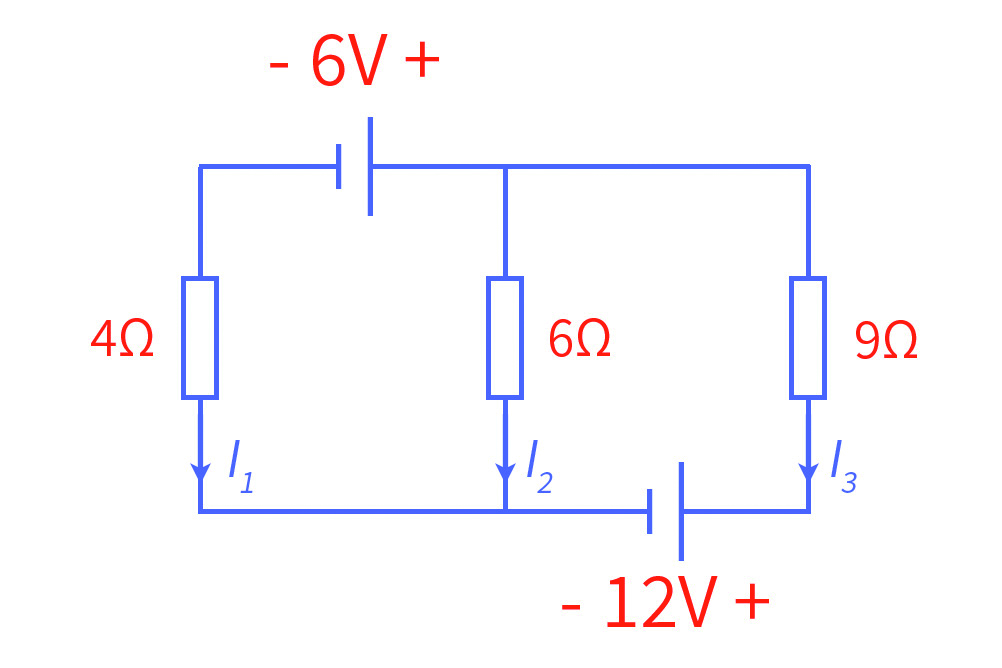
\includegraphics[scale = 0.25]{graphics/circuit.jpg}
\caption{\textit{The circuit for Exercise \ref{ex:circuitsys}.}}
\label{fig:circuitsys}
\end{figure}
\begin{Answer}
The first two equations below come from the left inner loop and right inner loop, but one of them can be replaced by the outer loop as well.
\begin{align*}
\left\{
\begin{alignedat}{2}
&-4I_1 + 6I_2& &= 6\\
&-6I_2 + 9I_3& &= -12\\
&I_1 + I_2 + I_3& &= 0
\end{alignedat}\right.
\end{align*}
and the solution is $I_1 = -\frac{3}{19}$, $I_2 = \frac{17}{19}$, $I_3 = -\frac{14}{19}$ (in Amperes).
\end{Answer}

\begin{Exercise}
\phantomsection
\label{ex:shallowwater}
The \index{Shallow Water Equations}\textit{shallow water equations} (see Figure \ref{fig:shallowwater}) describe the evolution of the gravity wave under some approximations such as \textit{hydrostatic balance} and a sufficiently shallow fluid depth, and have the form of
\begin{align}
\left\{\begin{alignedat}{2}
&\frac{\partial \eta}{\partial t} + H(\frac{\partial u}{\partial x} + \frac{\partial v}{\partial y})& &= 0 \\
&\frac{\partial u}{\partial t}& &= -g\frac{\partial \eta}{\partial x} \\
&\frac{\partial v}{\partial t}& &= -g\frac{\partial \eta}{\partial y} 
\end{alignedat}\right.
\end{align}
when the Coriolis effect is ignored. By assuming a traveling wave solution
\begin{align*}
u &= \tilde{U} \cos(kx + ly - \omega t) \\
v &= \tilde{V} \cos(kx + ly - \omega t) \\
\eta &= \tilde{\eta} \cos(kx + ly - \omega t)
\end{align*}
where $\tilde{U}$, $\tilde{V}$, $\tilde{\eta}$ are some constants to be determined, show that the equations will become
\begin{align}
\left\{\begin{alignedat}{2}
&\omega \tilde{\eta} - kH \tilde{U} - lH \tilde{V}& &= 0 \\
&\omega \tilde{U} - kg \tilde{\eta}& &= 0 \\
&\omega \tilde{V} - lg \tilde{\eta}& &= 0
\end{alignedat}\right.
\end{align}
By requiring that $\tilde{U}$, $\tilde{V}$, $\tilde{\eta}$ have a non-trivial solution so that they are not all zeros, derive the dispersion relation of gravity wave, which is
\begin{align*}
\omega^2 &= gH(k^2 + l^2) \\
\omega &= c\kappa
\end{align*}
where $c = \sqrt{gH}$ is the wave speed, and $\kappa = \sqrt{k^2 + l^2}$ is the total wavenumber.
\end{Exercise}
\begin{figure}[ht!]
\centering
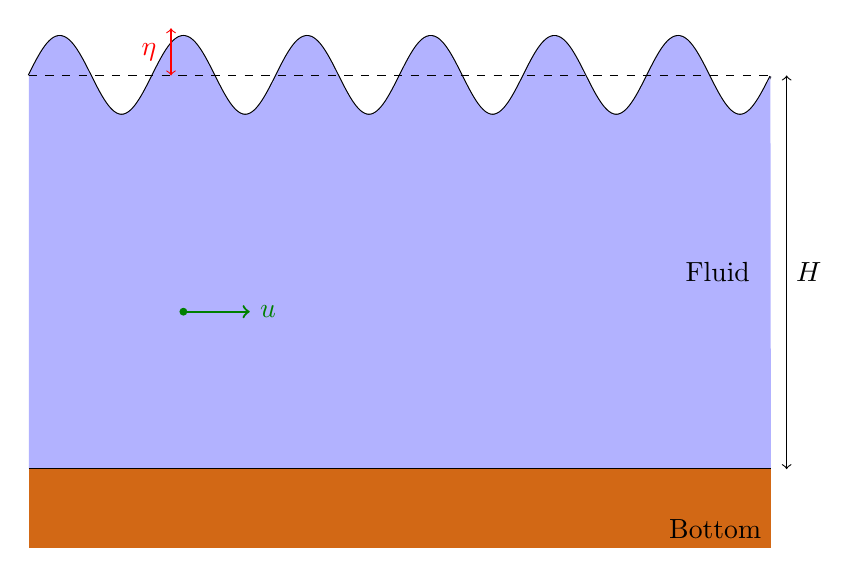
\begin{tikzpicture}
    \draw [thick,color=black,domain=0:3*pi,samples=500] plot (\x, {5+0.5*sin(deg(4*\x))});
    \fill [blue!30] (3*pi,0) -- (0,0) -- plot[domain=0:3*pi,samples=500]  (\x, {5+0.5*sin(deg(4*\x))});
    \draw [thick,color=black] (0,0) -- (3*pi, 0);
    \fill [Brown!50!Orange] (0,0) rectangle (3*pi, -1) node[above left, black]{Bottom};
    \draw [<->] (3*pi+0.2, 0) -- (3*pi+0.2, 5) node[midway, xshift=8]{$H$};
    \draw [<->,red] (0.575*pi, 5.6) -- (0.575*pi, 5) node[midway, xshift=-8]{$\eta$};
    \draw [dashed, black] (0, 5) -- (3*pi, 5);
    \fill [Green] (0.625*pi, 2) circle(.05);
    \draw [thick, Green, ->] (0.625*pi, 2) -- (0.575*pi+1, 2) node[right]{$u$};
    \node at (8.75, 2.5) {Fluid};
\end{tikzpicture}
\caption{\textit{The $x$-$z$ cross-section of shallow water system in Exercise \ref{ex:shallowwater}. $\eta$ is the height of free surface, $H$ is the mean depth of the fluid, and $u$ [$v$] is the fluid velocity along the $x$-axis [$y$-axis, into/out of the page].}}
\label{fig:shallowwater}
\end{figure}
\begin{Answer}
Substituting the given wave solution forms into the equation, we have
\begin{align*}
\begin{split}
&\omega\tilde{\eta}\sin(kx+ly-\omega t) + H(-k\tilde{U}\sin(kx+ly-\omega t) \\
&-l\tilde{V}\sin(kx+ly-\omega t)) = 0 \\    
\end{split} \\
&\omega\tilde{U}\sin(kx+ly-\omega t) = gk\tilde{\eta}\sin(kx+ly-\omega t) \\
&\omega\tilde{V}\sin(kx+ly-\omega t) = gl\tilde{\eta}\sin(kx+ly-\omega t)
\end{align*}
Cancelling out all the sine factors, we arrive at the linear system displayed in the question
\begin{align*}
\left\{\begin{alignedat}{2}
&\omega \tilde{\eta} - kH \tilde{U} - lH \tilde{V} & &= 0 \\
&\omega \tilde{U} - kg \tilde{\eta} & &= 0 \\
&\omega \tilde{V} - lg \tilde{\eta} & &= 0
\end{alignedat}\right.
\end{align*}
For $\tilde{U}$, $\tilde{V}$, $\tilde{\eta}$ to have a non-trivial solution other than all zeros, we require the determinant of the corresponding coefficient matrix to be zero according to Theorem \ref{thm:sqlinsysunique}, which leads to
\begin{align*}
\begin{vmatrix}
\omega & -kH & -lH \\
-kg & \omega & 0 \\
-lg & 0 & \omega
\end{vmatrix} &= 0 \\
\omega^3 - gHk^2\omega - gHl^2\omega &= 0 \\
\omega^2 - gH(k^2 + l^2) &= 0 
\end{align*}
as the dispersion relation of gravity wave.
\end{Answer}

\begin{Exercise}
Solve for the condensation height and temperature $z_{cd}$ and $T_{cd}$ in Exercise \ref{ex:lapse}.
\end{Exercise}
\begin{Answer}
$T_{cd} \approx \SI{15.9}{\celsius}$, $z_{cd} \approx \SI{0.97}{\km}$.
\end{Answer}

\begin{Exercise}
Solve the \textit{Chickens and Rabbits in the Same Cage} problem in Exercise \ref{ex:animals}. If we now introduce a new type of mystical creature who has one head and three legs, and throw them in another cage along with some chickens and rabbits, find all possible numbers of the three species if the cage now has $48$ heads and $122$ legs.
\end{Exercise}
\begin{Answer}
$x = 23$, $y = 12$. For the extra part, the new system of equations becomes (denote the number of third species as $z$)
\begin{align*}
\begin{bmatrix}
1 & 1 & 1 \\
2 & 4 & 3
\end{bmatrix}
\begin{bmatrix}
x \\
y \\
z
\end{bmatrix}
=
\begin{bmatrix}
48 \\
122
\end{bmatrix}
\end{align*}
By Gaussian Elimination, we have
\begin{align*}
\left[
\begin{array}{@{}ccc|c@{}}
1 & 1 & 1 & 48 \\
2 & 4 & 3 & 122
\end{array}
\right]
&\to
\left[
\begin{array}{@{}ccc|c@{}}
1 & 1 & 1 & 48 \\
0 & 2 & 1 & 26
\end{array}
\right] & R_2 - 2R_1 \to R_2 \\
&\to
\left[
\begin{array}{@{}ccc|c@{}}
1 & 1 & 1 & 48 \\
0 & 1 & \frac{1}{2} & 13
\end{array}
\right] & \frac{1}{2}R_2 \to R_2 \\
&\to
\left[
\begin{array}{@{}ccc|c@{}}
1 & 0 & \frac{1}{2} & 35 \\
0 & 1 & \frac{1}{2} & 13
\end{array}
\right] & R_1 - R_2 \to R_1
\end{align*}
Let $z = t$ as the free variable, then we have $y = 13 - \frac{1}{2}t$ and $x = 35-\frac{1}{2}t$, and hence
\begin{align*}
\begin{bmatrix}
x \\
y \\
z
\end{bmatrix}
=
\begin{bmatrix}
35-\frac{1}{2}t \\
13-\frac{1}{2}t \\
t
\end{bmatrix}
=
\begin{bmatrix}
35 \\
13 \\
0
\end{bmatrix}
+
t
\begin{bmatrix}
-\frac{1}{2} \\
-\frac{1}{2} \\
1
\end{bmatrix}
\end{align*}
Since the number of species must be a non-negative integer, the solution can be expressed in a more good-looking form of
\begin{align*}
\begin{bmatrix}
x \\
y \\
z
\end{bmatrix}
=
\begin{bmatrix}
35 \\
13 \\
0
\end{bmatrix}
+
s
\begin{bmatrix}
-1 \\
-1 \\
2
\end{bmatrix}
\end{align*}
where $s = \frac{t}{2}$, and the range of $s$ is $0, 1, \ldots, 13$ (when $s$ reaches $13$ there is no chicken remained).
\end{Answer}